\documentclass[tikz,border=3pt]{standalone}
% Shared style for every figure: one font (Latin Modern), one block vocabulary, token colours.
\usepackage{fontspec}
\usepackage{unicode-math}
\setmathfont{latinmodern-math.otf}
\usetikzlibrary{arrows.meta,positioning,fit,calc,backgrounds,shapes.misc,decorations.pathreplacing}
% Token colours: exact RGB codes, remapped to CSS variables after conversion (see tokens in svgfix.py)
\definecolor{ink}{RGB}{0,0,0}
\definecolor{inkb}{RGB}{90,90,90}
\definecolor{grid}{RGB}{200,200,200}
\definecolor{paper}{RGB}{255,255,255}
\definecolor{fdata}{RGB}{231,238,246}
\definecolor{fmodel}{RGB}{246,238,224}
\definecolor{ftarget}{RGB}{232,243,234}
\definecolor{fpub}{RGB}{248,233,226}
\definecolor{own}{RGB}{42,120,214}
\definecolor{pub}{RGB}{235,104,52}
\tikzset{
  >={Latex[length=1.9mm,width=1.5mm]},
  every picture/.style={line width=0.5pt, ink, font=\normalsize},
  blk/.style={draw=ink, rounded corners=1.2pt, align=center, inner xsep=5pt, inner ysep=4pt, minimum height=9mm, fill=paper},
  data/.style={blk, fill=fdata},
  model/.style={blk, fill=fmodel},
  target/.style={blk, fill=ftarget},
  pubm/.style={blk, fill=fpub},
  op/.style={draw=ink, circle, inner sep=1.2pt, fill=paper, font=\small},
  group/.style={draw=inkb, dashed, rounded corners=2pt, inner sep=6pt},
  glabel/.style={font=\small\scshape, text=inkb, inner sep=1pt},
  note/.style={font=\footnotesize, text=inkb, align=center, inner sep=1pt},
  wt/.style={font=\footnotesize, fill=paper, inner sep=1pt},
  flow/.style={->, draw=ink},
  dflow/.style={->, draw=inkb, dashed},
}

\begin{document}
\begin{tikzpicture}[font=\small]
\tikzset{blk/.append style={text width=2.75cm}}
\def\dx{3.35}
% inputs
\node[data] (rep)  at (0,2.75)  {Radiology reports\\[-1pt]{\footnotesize 4,407 studies}};
\node[data] (dcm)  at (0,-0.2) {MRI (DICOM)\\[-1pt]{\footnotesize 24,371 series}};
\node[data] (gold) at (0,-1.8) {Gold labels\\[-1pt]{\footnotesize 58 studies $\times$ 12}};
% label lane
\node[pubm] (llm)  at (\dx,2.75) {LLM label tables\\[-1pt]{\footnotesize 3 public sources}};
\node[pubm] (rap)  at (\dx,1.25) {Raptor teacher\\[-1pt]{\footnotesize public CoAtNet-2}};
\node[target] (tgt) at (2*\dx,1.95) {Training targets\\[-1pt]{\footnotesize $\tfrac12$ LLM $+$ $\tfrac12$ Raptor}};
% image lane
\node[blk] (cache) at (\dx,-0.2) {Slice cache\\[-1pt]{\footnotesize 6 slots, $102\times336^2$}};
\node[model] (train) at (2*\dx,-0.2) {Our models\\[-1pt]{\footnotesize ConvNeXt-T,\\[-2pt]EfficientNet-B3}};
\node[blk] (rank) at (3*\dx,-0.2) {Rank-mean\\[-1pt]{\footnotesize per finding}};
% outputs
\node[pubm] (pubs) at (3*\dx,2.75) {Public checkpoints\\[-1pt]{\footnotesize 5 models, 4 authors}};
\node[blk, line width=0.9pt] (fin) at (4*\dx,2.75) {Final picks\\[-1pt]{\footnotesize C19, C14\\[-2pt]public 0.958, private 0.942}};
\node[blk] (fork) at (4*\dx,1.15) {Forks\\[-1pt]{\footnotesize C3--C12, our leg at $\beta\le0.45$}};
\node[blk] (own) at (4*\dx,-0.35) {Own blend\\[-1pt]{\footnotesize B22\\[-2pt]public 0.945, private 0.932}};
% edges
\draw[flow] (rep) -- (llm);
\draw[flow] (llm.east) -| (tgt.north);
\draw[flow] (rap.east) -- ++(0.25,0) |- ([yshift=-1.5mm]tgt.west);
\draw[flow] (dcm.east) -- (cache.west);
\draw[flow] ([xshift=6mm]dcm.north) |- (rap.west);
\draw[flow] (cache) -- (train);
\draw[flow] (tgt) -- (train);
\draw[dflow] (gold.east) -| node[note, pos=0.25, above] {validation only} (train.south);
\draw[flow] (train) -- (rank);
\draw[flow] (rank.east) -- (rank.east -| own.west);
\draw[flow] (pubs) -- (fin);
\draw[flow] (rank.north) |- ([yshift=-1.5mm]fork.west);
\draw[flow] (pubs.south) |- ([yshift=1.5mm]fork.west);
% legend
\begin{scope}[shift={(0.0,-3.1)}]
  \foreach \st/\lab/\x in {data/input data/-1.2, pubm/public asset/1.95, model/trained by us/5.1, target/targets/8.25, blk/processing step/10.9}{
    \node[\st, text width=, minimum width=0.55cm, minimum height=0.32cm, inner sep=0pt] at (\x,0) {};
    \node[anchor=west, font=\footnotesize] at ({\x+0.4},0) {\lab};
  }
\end{scope}
\end{tikzpicture}
\end{document}
